\section{変更のモデル化}

Clojureの焦点はimmutableな値であることを思い出してください。不変のデータでは、"更新 "は、その場のエンティティまたはエンティティを更新するのではなく、エンティティ(またはエンティティのコレクション)の新しいインスタンスを生成します。ほとんどの場合、この方法で十分に目的を果たすことができます。時には、アプリケーションの世界の変化をモデル化し、データの変化を追跡する必要があります。具体的には、変更されたデータのセットへの参照を保持する必要があります。

マルチスレッドのシナリオでは、その場でデータを更新することは、多くの複雑な問題を引き起こします。誰がデータを変更できるのか?他のスレッドにはどのように変更が通知されるのか?複数の更新が同時に発生した場合、どのプロセスが優先されるのか?Clojureは、状態管理ツールによって、これらの質問すべてにエレガントな答えを提供します。これらのツールを効果的に使用するには、まずClojureのアイデンティティと状態へのアプローチを理解する必要があります。

\subsection{スナップショットで見る}

その理解を助けるために、少し時間の話をしましょう。人間の経験は連続的に見えますが、あなたの感覚は情報を個別の量子に分けて収集しています。音、景色、匂いは、それぞれ独立して脳に入り、時間的な瞬間に相関します。その瞬間が連続して再生されることで、連続した知覚が得られると錯覚しているのです。

もし、自分の視覚的な量子を見るなら、次の図に示すエドワード・マイブリッジの「疾走するサリー・ガードナー」のようなスナップショットの連続が見えるだろう。

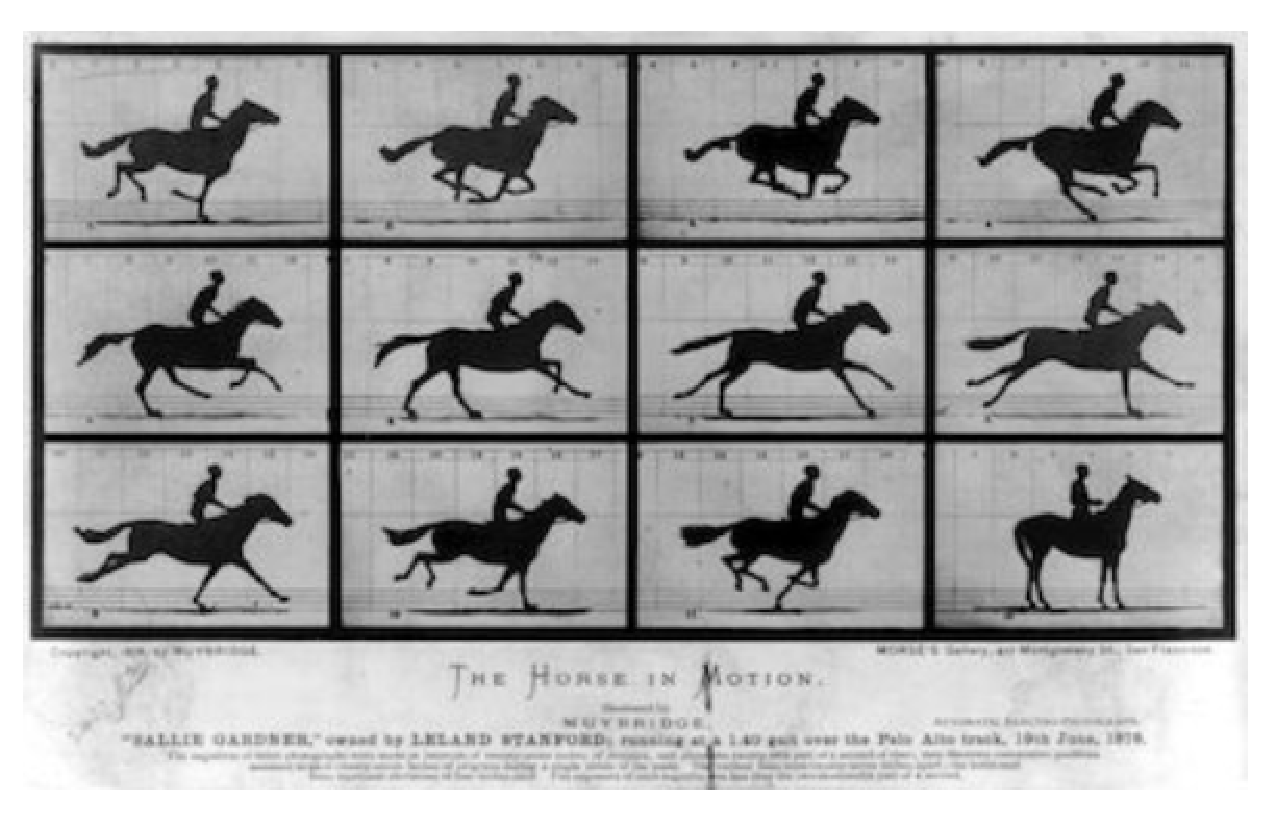
\includegraphics[width=10cm]{fig_04_001.eps}


マイブリッジが1878年に撮影した写真で、馬の4つの蹄が同時に地面から離れることがあるかどうかを調べるために撮影された。この写真に写し出された見かけ上の動きは幻想的なものだが、私たちの心には連続性がある。私たちはこの写真を順番に再生し、サリー・ガードナーの歴史的な走りを見ることができるのです。

このシリーズを、地面に到達したひづめの数を記録する存在として表現することを想像してみよう。最初の更新では蹄が1つ減り、2つ目はゼロ、そして最後の写真にたどり着くまで、この状態が続く。

もし、1つの値しか見えないのであれば、このシリーズの面白さは失われてしまいます。馬の動きがはっきりしないだけでなく、2枚目と3枚目を除いたすべてのフレームで、元の問題が解決されないままになってしまうのです。時間という次元を失ってしまうのだ。

同様に、オブジェクト指向のプログラマーとして変化するデータにアプローチする場合、世界のデータをオブジェクトとしてモデル化する傾向があります。世界が変われば、その世界を表現するオブジェクトも更新され、「今」を反映した世界のモデルが出来上がります。この方法の問題点は、視聴者に最後の1フレームしか残らないことです。

このような動作は、一連のステップの結果を1つのスレッドで処理する、つまり「今」を見るしかないシステムとして、まさに理想的と言えます。しかし、習慣的に「今」しか見ていないと、アイデンティティとステートという二つの概念を混同してしまいがちです。ここで、この2つの概念を少し整理してみよう。



\subsection{アイデンティティと状態の理解}

あなたのお気に入りのコーヒーショップを考えてみましょう。時間帯によって、開いていたり閉まっていたりします。新しい焙煎豆が入荷すると、提供されるコーヒーも変わります。シフトによって、エスプレッソマシンを操るバリスタも違えば、バーにいるお客さんも違います。コーヒーショップは、場所や名前さえも変わるかもしれません。このような変化があっても、コーヒーショップのアイデンティティは変わりません。コーヒー、客層、スタッフ、そしてモーニングコーヒーが必要なときにドアに鍵がかかっているかどうかなど、さまざまなものを包み込むのが店のアイデンティティです。

一方、ステートとは、ある瞬間のアイデンティティーの価値を表すものです。コーヒーショップに例えると、火曜日の午前7時、店はオープンし、リンジーがレジを管理し、ジミーがグラインダーを回し、お客はオフィスに向かう前にラップトップをチェックし、ライトローストはエチオピア産の何かだったとする。

朝のシフトを考えることで、ステートとアイデンティティが別物であることがわかる。状態とは、あるアイデンティティに属する価値観、あるいは価値観の集合のことである。アイデンティティは、時間によって区切られた一連の状態である。私たちは、どの瞬間にも、どの深煎りのコーヒーが提供されるのか、席は空いているのか、といった質問をすることがあります。という質問をするとき、正確な回答を得るためには、更新が整然と行われなければならず、そうでなければ、思いがけず誰かの膝の上に座ってしまうかもしれません。

このためには、ミュータビリティが必要なだけでなく、その更新が観察者の視点から離散的かつ瞬時に行われる必要がある。つまり、あるIDに対して、そのIDのデータに変更を加えることで、すべての観測者から同時に見えるようにする機能が必要なのです。


\subsection{連続した更新}

Clojureでは、更新したい値を持つIDへの参照を作成することができます。一般的に、参照は不変の値の連続のための変更可能なコンテナです。Clojureは、時間の経過とともに変化する値を管理するアプローチを統一更新モデルと呼びます。統一更新モデルは一般に次のような形式をとります。


\begin{lstlisting}[numbers=none]
(update-fn container data-fn & args)
\end{lstlisting}


この場合の\texttt{data-fn}は、現在リファレンスに格納されている値に適用され、新しい値を作成する。この新しい値は成功し、参照が保持している現在の値を置き換える。すべての参照型(\texttt{var},\texttt{atom},\texttt{agent},\texttt{ref})はこのモデルを用いて,連続したデータを実装する.しかし、それぞれの型は独自のセマンティクスを持っています。

それぞれのIDを保持するためにどの参照型を使うかは、更新にどのような特性を持たせたいかによります。とりあえず、アトミックな継承とトランザクションな継承に注目してみましょう。どちらも統一更新モデルを実装しています。これらのいずれの場合も、ID の値は常に読み取ることができます。


\subsubsection{アトミックサクセション(原子的継承)}

原子的継承は1つのIDを更新します。更新関数と ID が与えられると、その関数は ID の現在値に適用されます。うまくいけば、その結果が現在の値を置き換えます。update 関数の実行中に別のスレッドが ID の値を更新した場合、複雑な問題が発生する可能性があります。Clojureは、成功するか再試行回数制限に達するまで、新しい値に対して関数を再試行することで、これを処理します。

アトミックな継承は、システムの他の部分から独立して変更できるスタンドアロンな値(または複合値)があるときに使用されます。アトミックアップデートが完了すると、(ウォッチ関数を介して)他のシステムの値や関数に通知することができますが、保持する値は他のステートフル参照と調整する必要はありません。

コレクションは、インベントリ、従業員名簿、入力または出力チャネルのリストなど、アトミックな継承の良い候補になります。次の節では、インベントリを使った例を紹介します。

Clojureでは、アトム継承には同期と非同期の表現があり、それぞれアトムとエージェントで表現されます。アトムについてはこれから本題に入りますが、エージェントについてはここで説明します。

\subsubsection{トランザクション継承}

2つのIDを一緒に更新する必要がある場合は、トランザクション継承を使用することになります。その名が示すように、これにはトランザクションが含まれ、調整された更新のすべてまたはいずれかが起こるようにします。

一般に、トランザクションは一連のIDに対する一連の調整された変更で構成されます。1つのIDは同時に複数のトランザクションに関与することができます。アトミック継承と同様に、Clojureは多数の再試行によって競合を解決します。アトミック継承とは異なり、多くのIDが関与しているため、トランザクション全体が再試行されます。1つの独立したIDへの単一の更新ではなく、トランザクションは、いくつかの調整されたIDへの多くの更新を含むことができます。

\begin{itembox}[l]{トランザクションの内側}
トランザクションとは、アプリケーションの現実を表す小さな泡のようなものです。このバブルの中で、アイデンティティはあたかも ID から読み込まれた値は、トランザクションのタイムライン内では現在のものであり、更新を適用して値を調整することができます。

トランザクションが完了し、アプリケーションに変更をコミットする前に、Clojureはトランザクションに関与するアイデンティティのいずれかがバブルの外で更新されているかどうかを確認します。もし更新されていれば、そのIDの最新の値セットを読み込んで、トランザクションを再試行します。そうでなければ、トランザクションはコミットされ、バブルは弾けます。
\end{itembox}

Programming Clojure (2nd edition)を読んでいない人のために説明すると、Clojureは多版型同時実行制御(MVCC)モデルを実装したソフトウェア・トランザクション・メモリ(STM)を使用してこれを実現します。

ここまで、一般的な方法でアトミックとトランザクションの継承について話してきました。では、実際に使用できるツールとコードについて説明します。

